%PREENCHA OS CAMPOS ABAIXO COM AS INFORMAÇÕES DO SEU TRABALHO
%SUBSTITUA OS EXEMPLOS
\author{Leocádio Nestor Gumercindo Filho}
\title{A representação do arco-íris no Reino dos Unicórnios:\\ uma aplicação da variável CORES PRIMÁRIAS}
%Data da defesa. Apenas mês e ano.
\date{Jan. 2050}

%INFORMAÇÕES DA INSTITUIÇÃO E CURSO
\newcommand{\instituicao}{Instituto Federal de Pernambuco}
\newcommand{\campus}{Campus Garanhuns}
\newcommand{\curso}{Análise e desenvolvimento de sistemas}
\newcommand{\titulacao}{Tecnólogo}%Ou bacharel, ou licenciado.
\newcommand{\localdefesa}{Garanhuns - PE}
%Data exata da defesa para a folha de aprovação.
\newcommand{\dataexatadefesa}{01 de jan. \the\year}

%INFORMAÇÕES DO ORIENTADOR/A
\newcommand{\orientador}{Nome Completo do/a Orientador/a}
%Mude o texto da linha abaixo conforme o gênero do orientador/a.
\newcommand{\printorientador}{(Orientador/a)}
%Substitua "Titulação do orientador" por Esp., Me., Ma., Dr. ou Drª
\newcommand{\titorientador}{Dr.}
%Altere a linha abaixo caso seu orientador não seja do IFPE Garanhuns
\newcommand{\localorientador}{Instituto Federal de Pernambuco Campus Garanhuns}

%INFORMAÇÕES DOS AVALIADORES
%Avaliador/a 1
\newcommand{\avaliadorum}{Nome Completo do/a Avaliador/a 1}
\newcommand{\titavaliadorum}{Drª}% Esp., Me., Ma., Dr. ou Drª
\newcommand{\localavalum}{Universidade Floresta Mágica}% UFRPE, UFPE, UFMG etc por extenso
%Avaliador/a 2
\newcommand{\avaliadordois}{Nome Completo do/a Avaliador/a 1}
\newcommand{\titavaliadordois}{Me.}% Esp., Me., Ma., Dr. ou Drª
\newcommand{\localavaldois}{Instituto Bosque das Flores}% UFRPE, UFPE, UFMG etc por extenso

%FORMATAÇÃO DO ELEMENTOS PRÉ-TEXTUAIS - NÃO ALTERAR
%Capa
\begin{center}
%CAPA
%CASO NÃO DESEJE O LOGO DA INSTITUIÇÃO, EXCLUIR LINHA ABAIXO.

\includegraphics[scale=.10]{./img/logo-ifpe.png}\\
\textbf{\textsc{\instituicao}}\\
%Caso sua instituição não tenha CAMPUS, remova o comando \campus.
\textbf{\textsc{\campus}}\\
\textbf{\textsc{\curso}}


\vspace*{5cm}
\textbf{\thetitle}\\
\textbf{\theauthor}

\vspace*{\fill}
\localdefesa\\
\thedate
\end{center}

%FOLHA DE ROSTO + TIPO DE TRABALHO
\frontmatter{
\newpage
\thispagestyle{empty}
\begin{center}
    \textbf{\theauthor}
	
    \vspace*{5cm}
    \textbf{\thetitle}
\end{center}
%Caso sua instituição não tenha CAMPUS, remova o comando \campus.
%ATENÇÃO À PREPOSIÇÃO "AO/À"
\vspace*{2cm}
    \begin{textofolharosto}
    Trabalho de conclusão de curso apresentado ao/à \instituicao\ \campus\ como requisito parcial para obtenção do título de \titulacao\ em \curso.\\
    \ \\
    \textbf{Orientador:} \orientador
    \end{textofolharosto}

\begin{center}
\vspace*{\fill}
    \localdefesa\\
    \thedate
\end{center}

%FICHA CATALOGRÁFICA.
%Após a confecção da ficha catalográfica pela biblioteca de sua instituição --
%aqui, a biblioteca do IFPE Campus Garanhuns --
%imprima o arquivo (provavelmente em .docx) para pdf e salve-o
%na pasta pretxt do projeto com o nome "fichacatalografica.pdf".
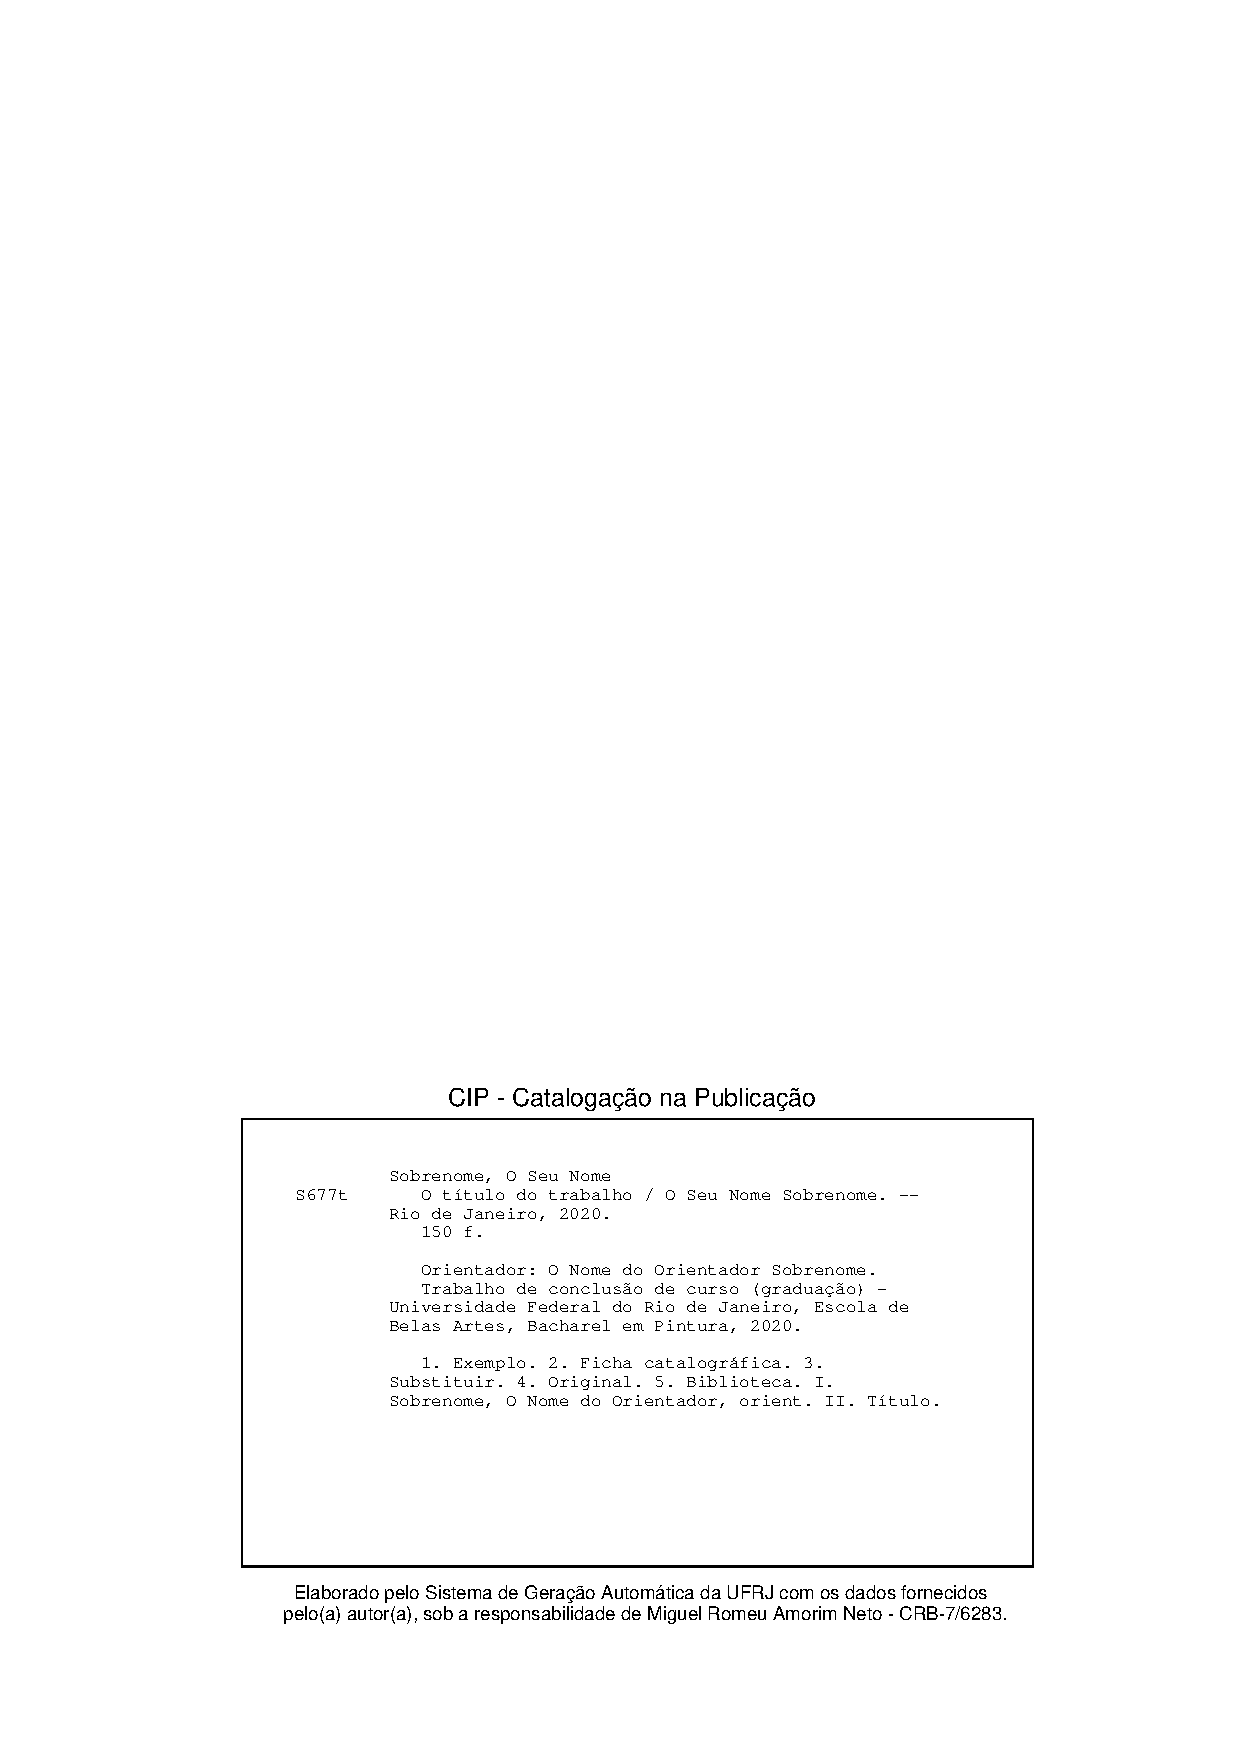
\includepdf{fichacatalografica.pdf}

%FOLHA DE APROVAÇÃO
\newpage
\thispagestyle{empty}
\begin{center}
    \textbf{\textsc{\theauthor}}
	
    \textbf{\textsc{\thetitle}}
%ATENÇÃO AO USO DA PREPOSIÇÃO (DO/DA) ANTES DO COMANDO \instituicao	
\vspace*{2cm}
    \begin{textofolharosto}
        Este Trabalho de Conclusão de Curso foi julgado adequado para obtenção do Título de \titulacao\ e aprovado em sua forma final pelo Curso de \curso\ da \instituicao\ \campus.\\
        \ \\
        \ \\
        \localdefesa\ \-- \dataexatadefesa
        \end{textofolharosto}
	
        \vspace*{2cm}
        \line(1,0){10cm}\\
        \textbf{\titorientador\ \orientador\ \printorientador}\\
        \localorientador\\
        	
        \vspace*{2cm}
        \line(1,0){10cm}\\
        \textbf{\titavaliadorum\ \avaliadorum}\\
        \localavalum\\
        	
        \vspace*{2cm}
        \line(1,0){10cm}\\
        \textbf{\titavaliadordois\ \avaliadordois}\\
        \localavaldois
    \end{center}

%EPÍGRAFE
\newpage
\thispagestyle{empty}
\vspace*{\fill}
\epigraph{\textit{Uma frase importante relacionada ao trabalho.}}{\textsc{Quem disse a frase.}}

%DEDICATÓRIA
\newpage
\thispagestyle{empty}
\vspace*{15cm}
\begin{flushright}
    \SingleSpacing\textit{Dedico este trabalho ao ilustríssimo Professor Dr. André Padilha por ter me fornecido esse modelo de trabalho em \LaTeX\ e facilitar minha jornada na escrita acadêmica.}
\end{flushright}

%AGRADECIMENTOS
\newpage
\pagestyle{empty}
\begin{center}
	\textbf{\textsc{Agradecimentos}}
\end{center}
% Digite os agradecimentos a partir da linha abaixo 
% e SEMPRE após o comando no indent, após o primeiro
% afradecimento. EXEMPLO:
Agradeço incomensuravelmente ao ilustríssimo Professor Dr. André Padilha por ter me fornecido esse modelo de trabalho em \LaTeX\ e facilitar minha jornada na escrita acadêmica.

\noindent Abaixo, o resto dos agradecimentos...

\noindent Ao papai.

\noindent À mamãe.

\noindent Ao meu papagaio José Eustáquio. 

\noindent Ao \textit{Lorem ipsum}, abaixo.

\noindent  \lipsum[10]

%RESUMO e ABSTRACT
\newpage
\pagestyle{empty}
\begin{center}
    \textbf{\textsc{Resumo}}
\end{center}
\SingleSpacing\noindent
    O resumo de um trabalho acadêmico é normatizado pela ABNT 6028:2018. Deve ser escrito em 3ª pessoa, ter entre 150 a 500 palavras e apresentar: \textit{finalidades (objetivos), metodologia, referencial teórico, resultados e conclusões}. Deve ser escrito em bloco único, com frases concisas. Para trabalhos de graduação, a prática mais comum é ter até 300 palavras.

\vspace*{0.5cm}
\noindent\textbf{Palavras-chave:} Palavra 1; Palavra 2; Palavra 3. (Até cinco, separadas por \q{ ; } (ponto e vírgula).

%ABSTRACT
\newpage
\pagestyle{empty}
\begin{center}
    \textbf{\textsc{Abstract}}
\end{center}
\SingleSpacing\noindent
    Write your abstract here. Follow the same rules as indicated previously. Avoid using any automatic translation tool as \textit{Google Translator} except if you know what you are doing.

\vspace*{0.5cm}
\noindent\textbf{Keywords:} Word 1; Word 2; Word 3.
}
\newpage\tableofcontents*
\thispagestyle{empty}
\newpage\listoffigures*
\thispagestyle{empty}
\newpage\listoftables*
\thispagestyle{empty}